% Options for packages loaded elsewhere
\PassOptionsToPackage{unicode}{hyperref}
\PassOptionsToPackage{hyphens}{url}
%
\documentclass[
]{article}
\usepackage{amsmath,amssymb}
\usepackage{lmodern}
\usepackage{iftex}
\ifPDFTeX
  \usepackage[T1]{fontenc}
  \usepackage[utf8]{inputenc}
  \usepackage{textcomp} % provide euro and other symbols
\else % if luatex or xetex
  \usepackage{unicode-math}
  \defaultfontfeatures{Scale=MatchLowercase}
  \defaultfontfeatures[\rmfamily]{Ligatures=TeX,Scale=1}
\fi
% Use upquote if available, for straight quotes in verbatim environments
\IfFileExists{upquote.sty}{\usepackage{upquote}}{}
\IfFileExists{microtype.sty}{% use microtype if available
  \usepackage[]{microtype}
  \UseMicrotypeSet[protrusion]{basicmath} % disable protrusion for tt fonts
}{}
\makeatletter
\@ifundefined{KOMAClassName}{% if non-KOMA class
  \IfFileExists{parskip.sty}{%
    \usepackage{parskip}
  }{% else
    \setlength{\parindent}{0pt}
    \setlength{\parskip}{6pt plus 2pt minus 1pt}}
}{% if KOMA class
  \KOMAoptions{parskip=half}}
\makeatother
\usepackage{xcolor}
\usepackage[margin=1in]{geometry}
\usepackage{color}
\usepackage{fancyvrb}
\newcommand{\VerbBar}{|}
\newcommand{\VERB}{\Verb[commandchars=\\\{\}]}
\DefineVerbatimEnvironment{Highlighting}{Verbatim}{commandchars=\\\{\}}
% Add ',fontsize=\small' for more characters per line
\usepackage{framed}
\definecolor{shadecolor}{RGB}{248,248,248}
\newenvironment{Shaded}{\begin{snugshade}}{\end{snugshade}}
\newcommand{\AlertTok}[1]{\textcolor[rgb]{0.94,0.16,0.16}{#1}}
\newcommand{\AnnotationTok}[1]{\textcolor[rgb]{0.56,0.35,0.01}{\textbf{\textit{#1}}}}
\newcommand{\AttributeTok}[1]{\textcolor[rgb]{0.77,0.63,0.00}{#1}}
\newcommand{\BaseNTok}[1]{\textcolor[rgb]{0.00,0.00,0.81}{#1}}
\newcommand{\BuiltInTok}[1]{#1}
\newcommand{\CharTok}[1]{\textcolor[rgb]{0.31,0.60,0.02}{#1}}
\newcommand{\CommentTok}[1]{\textcolor[rgb]{0.56,0.35,0.01}{\textit{#1}}}
\newcommand{\CommentVarTok}[1]{\textcolor[rgb]{0.56,0.35,0.01}{\textbf{\textit{#1}}}}
\newcommand{\ConstantTok}[1]{\textcolor[rgb]{0.00,0.00,0.00}{#1}}
\newcommand{\ControlFlowTok}[1]{\textcolor[rgb]{0.13,0.29,0.53}{\textbf{#1}}}
\newcommand{\DataTypeTok}[1]{\textcolor[rgb]{0.13,0.29,0.53}{#1}}
\newcommand{\DecValTok}[1]{\textcolor[rgb]{0.00,0.00,0.81}{#1}}
\newcommand{\DocumentationTok}[1]{\textcolor[rgb]{0.56,0.35,0.01}{\textbf{\textit{#1}}}}
\newcommand{\ErrorTok}[1]{\textcolor[rgb]{0.64,0.00,0.00}{\textbf{#1}}}
\newcommand{\ExtensionTok}[1]{#1}
\newcommand{\FloatTok}[1]{\textcolor[rgb]{0.00,0.00,0.81}{#1}}
\newcommand{\FunctionTok}[1]{\textcolor[rgb]{0.00,0.00,0.00}{#1}}
\newcommand{\ImportTok}[1]{#1}
\newcommand{\InformationTok}[1]{\textcolor[rgb]{0.56,0.35,0.01}{\textbf{\textit{#1}}}}
\newcommand{\KeywordTok}[1]{\textcolor[rgb]{0.13,0.29,0.53}{\textbf{#1}}}
\newcommand{\NormalTok}[1]{#1}
\newcommand{\OperatorTok}[1]{\textcolor[rgb]{0.81,0.36,0.00}{\textbf{#1}}}
\newcommand{\OtherTok}[1]{\textcolor[rgb]{0.56,0.35,0.01}{#1}}
\newcommand{\PreprocessorTok}[1]{\textcolor[rgb]{0.56,0.35,0.01}{\textit{#1}}}
\newcommand{\RegionMarkerTok}[1]{#1}
\newcommand{\SpecialCharTok}[1]{\textcolor[rgb]{0.00,0.00,0.00}{#1}}
\newcommand{\SpecialStringTok}[1]{\textcolor[rgb]{0.31,0.60,0.02}{#1}}
\newcommand{\StringTok}[1]{\textcolor[rgb]{0.31,0.60,0.02}{#1}}
\newcommand{\VariableTok}[1]{\textcolor[rgb]{0.00,0.00,0.00}{#1}}
\newcommand{\VerbatimStringTok}[1]{\textcolor[rgb]{0.31,0.60,0.02}{#1}}
\newcommand{\WarningTok}[1]{\textcolor[rgb]{0.56,0.35,0.01}{\textbf{\textit{#1}}}}
\usepackage{graphicx}
\makeatletter
\def\maxwidth{\ifdim\Gin@nat@width>\linewidth\linewidth\else\Gin@nat@width\fi}
\def\maxheight{\ifdim\Gin@nat@height>\textheight\textheight\else\Gin@nat@height\fi}
\makeatother
% Scale images if necessary, so that they will not overflow the page
% margins by default, and it is still possible to overwrite the defaults
% using explicit options in \includegraphics[width, height, ...]{}
\setkeys{Gin}{width=\maxwidth,height=\maxheight,keepaspectratio}
% Set default figure placement to htbp
\makeatletter
\def\fps@figure{htbp}
\makeatother
\setlength{\emergencystretch}{3em} % prevent overfull lines
\providecommand{\tightlist}{%
  \setlength{\itemsep}{0pt}\setlength{\parskip}{0pt}}
\setcounter{secnumdepth}{-\maxdimen} % remove section numbering
\ifLuaTeX
  \usepackage{selnolig}  % disable illegal ligatures
\fi
\IfFileExists{bookmark.sty}{\usepackage{bookmark}}{\usepackage{hyperref}}
\IfFileExists{xurl.sty}{\usepackage{xurl}}{} % add URL line breaks if available
\urlstyle{same} % disable monospaced font for URLs
\hypersetup{
  pdftitle={Homework 2: Neo Lee},
  hidelinks,
  pdfcreator={LaTeX via pandoc}}

\title{Homework 2: Neo Lee}
\usepackage{etoolbox}
\makeatletter
\providecommand{\subtitle}[1]{% add subtitle to \maketitle
  \apptocmd{\@title}{\par {\large #1 \par}}{}{}
}
\makeatother
\subtitle{Introduction to Time Series, Fall 2023}
\author{}
\date{\vspace{-2.5em}Due Thursday September 21 at 5pm}

\begin{document}
\maketitle

The total number of points possible for this homework is 35. The number
of points for each question is written below, and questions marked as
``bonus'' are optional. Submit the \textbf{knitted html file} from this
Rmd to Gradescope.

If you collaborated with anybody for this homework, put their names
here:

\hypertarget{simple-regression}{%
\section{Simple regression}\label{simple-regression}}

\begin{enumerate}
\def\labelenumi{\arabic{enumi}.}
\tightlist
\item
  (2 pts) Derive the population least squares coefficients, which solve
  \[
  \min_{\beta_1, \beta_0} \, \mathbb{E} \big[ (y - \beta_0 - \beta_1 x)^2 \big],
  \] by differentiating the criterion with respect to each \(\beta_j\),
  setting equal to zero, and solving. Repeat the calculation but without
  intercept (without the \(\beta_0\) coefficient in the model).
\end{enumerate}

SOLUTION GOES HERE

\textbf{With intercept:}

Define \[Q := \mathbb{E} \big[ (y - \beta_0 - \beta_1 x)^2 \big].\] Then
we find \(\beta_0\) by setting \begin{align*}
    \frac{\partial Q}{\partial \beta_0} = \mathbb{E} \big[2 (\beta_0 + \beta_1 x - y) \big] & = 0 \\
    2 \mathbb{E}\big[\beta_0 \big] + 2 \mathbb{E}\big[\beta_1 x \big] - 
    2 \mathbb{E}\big[y \big] & = 0 \\
    \beta_0 + \beta_1 \mu_x - \mu_y & = 0 \\
    \underline{\beta_0} & = \mu_y - \beta_1 \mu_x.
\end{align*} Then, we find \(\beta_1\) by setting \begin{align*}
    \frac{\partial Q}{\partial \beta_1} = \mathbb{E} \big[2 x (\beta_0 + \beta_1 x - y) \big] & = 0 \\
    \beta_0\mathbb{E}\big[y \big] + \beta_1\mathbb{E}\big[x^2 \big] - \mathbb{E}\big[xy \big] & = 0 \\
    \beta_0\mu_x + \beta_1\left(Var(x)+\mu_x^2\right) - \left(Cov(x,y) + \mu_x\mu_y\right) & = 0 \\
    (\mu_y - \mu_x\beta_1)\mu_x + \beta_1Var(x) + \beta_1\mu_x^2 - Cov(x,y) - \mu_x\mu_y & = 0 \\
    \beta_1Var(x) - Cov(x,y) & = 0 \\
    \underline{\beta_1} & = \frac{Cov(x,y)}{Var(x)}.
\end{align*}

\textbf{Without intercept:}

Define \[Q:=\mathbb{E}\left[(y-\beta_1x)^2\right].\] Then we have
\begin{align*}
    \frac{\partial Q}{\partial \beta_1} = \mathbb{E} \big[2 x (\beta_1 x - y) \big] & = 0 \\
    \beta_1\mathbb{E}\big[x^2 \big] - \mathbb{E}\big[xy \big] & = 0 \\
    \beta_1\left(Var(x)+\mu_x^2\right) - \left(Cov(x,y) + \mu_x\mu_y\right) & = 0 \\
    \underline{\beta_1} & = \frac{Cov(x,y)+\mu_x\mu_y}{Var(x)+\mu_x^2}.
\end{align*}

\begin{enumerate}
\def\labelenumi{\arabic{enumi}.}
\setcounter{enumi}{1}
\tightlist
\item
  (2 pts) As in Q1, now derive the sample least squares coefficients,
  which solve \[
  \min_{\beta_1, \beta_0} \, \sum_{i=1}^n (y_i - \beta_0 - \beta_1 x_i)^2.
  \] Again, repeat the calculation but without intercept (no \(\beta_0\)
  in the model).
\end{enumerate}

SOLUTION GOES HERE

\textbf{With intercept:}

Define \[Q := \sum_{i=1}^n (y_i - \beta_0 - \beta_1 x_i)^2.\]

To find \(\beta_0\), we set \begin{align*}
    \frac{\partial Q}{\partial \beta_0} = \sum 2(\beta_1x_i+\beta_0-y_i) & = 0 \\
    \sum\beta_1x_i + n\beta_0-\sum y_i & = 0 \\
    \beta_1\frac{1}{n}\sum x_i + \beta_0 - \frac{1}{n}\sum y_i & = 0 \\
    \beta_0 & = \frac{1}{n}\sum y_i - \beta_1\frac{1}{n}\sum x_i \\
    \beta_0 & = \bar{y} - \beta_1\bar{x}.
\end{align*}

To find \(\beta_1\), we set \begin{align*}
    \frac{\partial Q}{\partial \beta_0} = \sum 2x(\beta_1x_i+\beta_0-y_i) & = 0 \\
    \beta_1\sum x_i^2+\beta_0\sum x_i - \sum x_iy_i & = 0 \\
    \beta_1\sum x_i^2 + \left(\bar{y} - \beta_1\bar{x}\right)\sum x_i - \sum x_iy_i & = 0 \\
    \beta_1\sum x_i^2 + \bar{y}\sum x_i - \beta_1\bar{x}\sum x_i - \sum x_iy_i & = 0 \\
    \beta_1\left(\sum x_i^2 - \bar{x}\sum x_i\right) & = \sum x_iy_i - \bar{y}\sum x_i \\
    \beta_1 & = \frac{\sum x_iy_i - \bar{y}\sum x_i}{\sum x_i^2 - \bar{x}\sum x_i}.
\end{align*}

Now, we take apart the numerator and denominator of \(\beta_1\):
\begin{align*}
    \sum x_iy_i - \bar{y}\sum x_i & = \sum (x_iy_i) - \bar{y}\cdot n\bar{x} \\
    & = \sum (x_iy_i) - \bar{y}\cdot n\bar{x}  - \bar{x}\cdot n\bar{y} + n\bar{x}\bar{y} \\
    & = \sum (x_iy_i) - \bar{y}\sum x_i - \bar{x}\sum y_i + n\bar{x}\bar{y} \\
    & = \sum\left(x_iy_i - x_i\bar{y} - \bar{x}y_i + \bar{x}\bar{y}\right) \\
    & = \sum(x_i-\bar{x})(y_i-\bar{y}); \\
    \sum x_i^2 - \bar{x}\sum x_i & = \sum x_i^2 - \bar{x}\cdot n\bar{x} \\
    & = \sum x_i^2 - \bar{x}\cdot n\bar{x} - \bar{x}\cdot n\bar{x} + \bar{x}\cdot n\bar{x} \\
    & = \sum x_i^2 - \bar{x}\sum x_i - \bar{x}\sum x_i + n\bar{x}^2 \\
    & = \sum\left(x_i^2 - 2x_i\bar{x} + \bar{x}^2\right) \\
    & = \sum(x_i-\bar{x})^2.
\end{align*}

Hence, \begin{align*}
    \beta_1 & = \frac{\sum_{i=1}^n(x_i-\bar{x})(y_i-\bar{y})}{\sum_{i=1}^n(x_i-\bar{x})^2}.
\end{align*}

\textbf{Without intercept:}

Define \[Q:=\sum_{i=1}^n(y_i-\beta_1x_i)^2.\]

To find \(\beta_1\), we set \begin{align*}
    \frac{\partial Q}{\partial \beta_1} = \sum 2x(\beta_1x_i-y_i) & = 0 \\
    \beta_1\sum x_i^2 - \sum x_iy_i & = 0 \\
    \beta_1 & = \frac{\sum x_iy_i}{\sum x_i^2}.
\end{align*}

\begin{enumerate}
\def\labelenumi{\arabic{enumi}.}
\setcounter{enumi}{2}
\tightlist
\item
  (2 pts) Prove of disprove: in the model without intercept, is the
  regression coefficient of \(x\) on \(y\) the inverse of that from the
  regression of \(y\) on \(x\)? Answer the question for each of the the
  population and sample versions.
\end{enumerate}

SOLUTION GOES HERE

\textbf{Population version:}

We are interested in knowing whether \(\beta_{y|x} = \beta_{x|y}^{-1}\)
in a model without intercept. We can check this by multiplying
\(\beta_{y|x}\) and \(\beta_{x|y}\) and check if the result is 1.
\begin{align*}
    \beta_{y|x} \times \beta_{x|y} & = \frac{Cov(x,y)+\mu_x\mu_y}{Var(x)+\mu_x^2} 
    \times \frac{Cov(x,y)+\mu_x\mu_y}{Var(y)+\mu_y^2} \\
    & = \frac{\mathbb{E}\left[xy\right]^2}{\mathbb{E}\left[x^2\right]\mathbb{E}\left[y^2\right]} \\
    & = \frac{\mathbb{E}\left[(xy)^2\right]-Var(xy)}{\mathbb{E}\left[x^2\right]\mathbb{E}\left[y^2\right]} \\
    & = \frac{Cov(x,y)+\mathbb{E}\left[x^2\right]\mathbb{E}\left[y^2\right]-Var(xy)}{\mathbb{E}\left[x^2\right]\mathbb{E}\left[y^2\right]}.
\end{align*}

Hence, it is only true when \(Cov(x,y)=Var(xy)=0\), and is not true in
general.

\textbf{Sample version:}

Similarly, we proceed by multiplying \(\beta_{y|x}\) and \(\beta_{x|y}\)
and check if the result is 1. \begin{align*}
    \beta_{y|x} \times \beta_{x|y} & = \frac{\sum x_iy_i}{\sum x_i^2} \times \frac{\sum x_iy_i}{\sum y_i^2}.
\end{align*} We can see easily that the product is not 1 in general.
Arbitrarily, take \((1,2)\) for \(i=1\) and \((3,4)\) for \(i=2\), the
product is 0.98.

\begin{enumerate}
\def\labelenumi{\arabic{enumi}.}
\setcounter{enumi}{3}
\tightlist
\item
  (3 pts) Consider the following hypothetical. Let \(y\) be the height
  of a child and \(x\) be the height of their parent, and consider a
  regression of \(y\) on \(x\), performed in in a large population.
  Suppose that we estimate the regression coefficients separately for
  male and female parents (two separate regressions) and we find that
  the slope coefficient from the former regression
  \(\hat\beta_1^{\text{dad}}\) is smaller than that from the latter
  \(\hat\beta_1^{\text{mom}}\). Suppose however that we find (in this
  same population) the sample correlation between a father's height and
  their child's height is \emph{larger} than that between a mother's
  height and their child's height. What is a plausible explanation for
  what is happening here?
\end{enumerate}

SOLUTION GOES HERE

Consider a model with intercept, \begin{align*}
    \hat{\beta}_1 & = \frac{\sum_{i=1}^n(x_i-\bar{x})(y_i-\bar{y})}{\sum_{i=1}^n(x_i-\bar{x})^2} \\
    & = \frac{\sum_{i=1}^n(x_i-\bar{x})(y_i-\bar{y})}{\sqrt{\sum_{i=1}^n(x_i-\bar{x})^2}\sqrt{\sum_{i=1}^{n}(y_i-\bar{y})^2}}\times 
    \frac{\sqrt{\sum_{i=1}^{n}(y_i-\bar{y})^2}}{\sqrt{\sum_{i=1}^{n}(x_i-\bar{x})^2}},
\end{align*} which is represented by the sample correlation times the
ratio of response sample standard deviations over predictor sample
standard deviations.

Therefore, one plausible explanation is that the sample standard
deviation of father's height is significantly larger than that of
mother's height. Hence, even the correlation between a father's height
and their child's height is larger, the standard deviation of father's
height may rescale \(\hat{\beta}_1^{\text{dad}}\) to a smaller value
than \(\hat{\beta}_1^{\text{mom}}\).

\hypertarget{multiple-regression}{%
\section{Multiple regression}\label{multiple-regression}}

\begin{enumerate}
\def\labelenumi{\arabic{enumi}.}
\setcounter{enumi}{4}
\tightlist
\item
  (2 pts) In class, we claimed that the multiple regression
  coefficients, with respect to responses \(y_i\) and feature vectors
  \(x_i \in \mathbb{R}^p\), \(i = 1,\dots,n\), can be written in two
  ways: the first is \[
  \hat\beta = \bigg( \sum_{i=1}^n x_i x_i^T \bigg)^{-1} \sum_{i=1}^n x_i y_i.
  \] The second is \[
  \hat\beta = (X^T X)^{-1} X^T y,
  \] where \(X \in \mathbb{R}^{n \times p}\) is a feature matrix, with
  \(i^{\text{th}}\) row \(x_i\), and \(y \in \mathbb{R}^n\) is a
  response vector, with \(i^{\text{th}}\) component \(y_i\). Prove that
  these two expressions are equivalent.
\end{enumerate}

SOLUTION GOES HERE

We first show that
\[\left(\sum_{i=1}^{n}x_ix_i^T\right)^{-1} = \left(X^TX\right)^{-1},\]
then we show that \[\sum_{i=1}^{n}x_iy_i = X^Ty.\]

\textbf{Notation:} Denote \(x_j^{(i)}\) as the \(j\)-th feature of the
feature vector \(\vec{x}\) at time step \(i\). The subscript is the
feature index, and the superscript is the time step index. We rewrite
the equation as
\[\left(\sum_{i=1}^{n}x^{(i)}x^{(i)^T}\right)^{-1} = \left(X^TX\right)^{-1}\]
to align with our notation.

We first check \(\sum_{i=1}^{n}x^{(i)}x^{(i)^T}\). For each time step
\(i\), \(x^{(i)}x^{(i)^T}\) will produce a \(p\times p\) matrix, denote
\(\mathcal{P}^{(i)}\), where
\[\mathcal{P}_{k,l}^{(i)} = x_k^{(i)}\cdot x_l^{(i)}.\] Hence, the
summation \(\sum_{i=1}^{n}x^{(i)}x^{(i)^T} = \mathcal{P}\) is a
\(p\times p\) matrix of sum of all \(\mathcal{P}^{(i)}\), for which
\[\mathcal{P}_{k,l} = \sum_{i=1}^{n}x_k^{(i)}\cdot x_l^{(i)}.\]

Now, we check \(X^TX\), denote \(\mathcal{P}^*\). \(X^T\) is a
\(p\times n\) matrix, and \(X\) is a \(n\times p\) matrix, so indeed
their product will produce a \(p\times p\) matrix. Notice the \(k\)-th
row of \(X^T\) represents the \(k\)-th feature vector of all \(n\) time
steps, which means
\[X^T_{k,\cdot} = \left[x_k^{(1)}, x_k^{(2)}, \cdots, x_k^{(n)}\right].\]
The \(l\)-th column of \(X\) represents the \(l\)-th feature of all
\(n\) time steps, which means \[X_{\cdot,l} = \begin{bmatrix}
    x_{l}^{(1)} \\
    x_{l}^{(2)} \\
    \vdots \\
    x_{l}^{(n)}
  \end{bmatrix}.\] Hence, the \(k,l\)-th entry of \(X^TX\) is
\begin{align*}
    \mathcal{P}^*_{k,l} & = X^T_{k,\cdot}X_{\cdot,l} \\
    & = x_k^{(1)}x_l^{(1)} + x_k^{(2)}x_l^{(2)} + \cdots + x_k^{(n)}x_l^{(n)} \\
    & = \sum_{i=1}^{n}x_k^{(i)}\cdot x_l^{(i)},
\end{align*} and we can see that
\(\mathcal{P}^* = \mathcal{P}\Rightarrow\mathcal{P}^{*^{-1}} = \mathcal{P}^{-1}\),
which means
\(\left(\sum_{i=1}^{n}x^{(i)}x^{(i)^T}\right)^{-1} = \left(X^TX\right)^{-1}\).

Next, we show \[\sum_{i=1}^{n}x_iy_i = X^Ty.\] Again, we rewrite the
equation to match our notation: \[\sum_{i=1}^{n}x^{(i)}y^{(i)} = X^Ty.\]
For each \(i\), \begin{align*}
    x^{(i)}y^{(i)} & = 
    \begin{bmatrix}
        x_1^{(i)} \\
        x_2^{(i)} \\
        \vdots \\
        x_p^{(i)}
      \end{bmatrix}y^{(i)} = 
    \begin{bmatrix}
        x_1^{(i)}y^{(i)} \\
        x_2^{(i)}y^{(i)} \\
        \vdots \\
        x_p^{(i)}y^{(i)}
      \end{bmatrix}
\end{align*} Hence, \(\sum_{i=1}^{n}x^{(i)}y^{(i)}\) is a \(p\times 1\)
vector, denote \(\vec{v}\), and the \(k\)-th entry
\[\vec{v}_k = \sum_{i=1}^{n}x_k^{(i)}y^{(i)}.\]

Now we check \(X^Ty\). \(X^T\) is a \(p\times n\) matrix, and \(y\) is a
\(n\times 1\) vector, so indeed their product will produce a
\(p\times 1\) vector, denote \(\vec{v}^*\). Notice the \(k\)-th row of
\(X^T\) represents the \(k\)-th feature vector of all \(n\) time steps,
which means
\[X^T_{k,\cdot} = \left[x_k^{(1)}, x_k^{(2)}, \cdots, x_k^{(n)}\right].\]
\(y\) is a vector of all \(n\) time steps, which means
\[y = \begin{bmatrix}
    y^{(1)} \\
    y^{(2)} \\
    \vdots \\
    y^{(n)}
  \end{bmatrix}.\] Indeed, the \(k\)-th entry of \(\vec{v}^*\) is
\begin{align*}
    \vec{v}^*_k & = X^T_{k,\cdot}y \\
    & = x_k^{(1)}y^{(1)} + x_k^{(2)}y^{(2)} + \cdots + x_k^{(n)}y^{(n)} \\
    & = \sum_{i=1}^{n}x_k^{(i)}y^{(i)}.
\end{align*} Therefore, \(\vec{v}^* = \vec{v}\), which means
\(\sum_{i=1}^{n}x^{(i)}y^{(i)} = X^Ty\).

\begin{enumerate}
\def\labelenumi{\arabic{enumi}.}
\setcounter{enumi}{5}
\tightlist
\item
  (Bonus) Derive the population and sample multiple regression
  coefficients by solving the corresponding least squares problem
  (differentiating the criterion with respect to each \(\beta_j\),
  setting equal to zero, and solving). For the sample least squares
  coefficient, deriving either representation in Q5 will be fine.
\end{enumerate}

SOLUTION GOES HERE

\hypertarget{marginal-multiple-connection}{%
\section{Marginal-multiple
connection}\label{marginal-multiple-connection}}

\begin{enumerate}
\def\labelenumi{\arabic{enumi}.}
\setcounter{enumi}{6}
\tightlist
\item
  (1 pts) Consider the simple linear regression of a generic response
  \(y_i\) on a constant predictor \(x_i = 1\), \(i = 1,\dots,n\),
  without intercept. Give the exact form of the sample regression
  coefficient.
\end{enumerate}

SOLUTION GOES HERE

Reusing the formula we derived from question 2, we have
\[\hat{\beta}_1 = \frac{\sum_{i=1}^{n}x_iy_i}{\sum_{i=1}^{n}x_i^2}.\]
Taking \(x_i = 1\) for all \(i\),
\[\hat{\beta}_1 = \frac{\sum_{i=1}^{n}y_i}{\sum_{i=1}^{n}1} = \frac{\sum_{i=1}^{n}y_i}{n} = \bar{y}.\]

\begin{enumerate}
\def\labelenumi{\arabic{enumi}.}
\setcounter{enumi}{7}
\item
  (3 pts) Recall the connection between multiple and marginal regression
  coefficients, as covered in lecture: the \(j^{\text{th}}\) multiple
  regression coefficient can be written in general as \[
  \hat\beta_j = \frac{(\hat{x}^{-j}_j)^T \hat{y}^{-j}}
  {(\hat{x}^{-j}_j)^T \hat{x}^{-j}_j},
  \] which we interpret as the simple linear regression coefficient of
  \(\hat{y}^{-j}\) on \(\hat{x}^{-j}\). These are \(y\) and \(x_j\),
  respectively, after we regress out the contributions of all other
  features. (See the lecture notes for the precise details.)

  Now note that we can treat a simple linear regression with an
  intercept term as a multiple regression with two features, with the
  first feature just equal to the constant 1. Using the above formula,
  and the answer from Q7, re-derive the expression for the slope in the
  simple linear model with intercept: \[
  \hat\beta_1 = \frac{\sum_{i=1}^n (x_i - \bar{x}) (y_i - \bar{y})} 
    {\sum_{i=1}^n (x_i - \bar{x})^2}.
  \]
\end{enumerate}

SOLUTION GOES HERE

Let's first find \(\hat{x}_j^{-j}\) and \(\hat{y}^{-j}\).

Notation: Denote \(x_0\) as the constant feature vector, and \(x_1\) as
the actual meaningful feature vector. We will take \(j = 1\) for the
rest of this problem. Any superscript \(^{-j}\) will mean dropping
\(x_1\), and this is not to be confused with \(^{-1}\), the inverse.

\(\hat{x}_1^{-j}\) is the residual of regressing \(x_1\) on \(X^{-j}\).
Note: \(X^{-j}\) is essentially \(x_0\). From question 7, we know that
\[\hat{\beta}_{x_1|x_0} = \bar{x}_1.\] Hence, the residual of regressing
\(x_1\) on \(X^{-j}\) is \begin{align*}
    \hat{x}_1^{-j} & = x_1 - x_0\hat{\beta}_{x_1|x_0} \\
    & = x_1 - x_0\bar{x}_1 \\
    & = \begin{bmatrix}
        x_1^{(1)} - \bar{x}_1 \\
        x_1^{(2)} - \bar{x}_1 \\
        \vdots \\
        x_1^{(n)} - \bar{x}_1 
    \end{bmatrix}
\end{align*}

\(\hat{y}^{-j}\) is the residual of regressing \(y\) on \(X^{-j}\).
Note: \(X^{-j}\) is essentially \(x_0\). From question 7, we know that
\[\hat{\beta}_{y|x_0} = \bar{y}.\] Hence, the residual of regressing
\(y\) on \(X^{-j}\) is \begin{align*}
    \hat{y}^{-j} & = y - x_0\hat{\beta}_{y|x_0} \\
    & = y - x_0\bar{y} \\
    & = \begin{bmatrix}
        y^{(1)} - \bar{y} \\
        y^{(2)} - \bar{y} \\
        \vdots \\
        y^{(n)} - \bar{y} 
    \end{bmatrix}
\end{align*}

Now, we put everything together. \begin{align*}
    \hat{\beta}_{1, (y|x_1)} & = \frac{\left(\hat{x}_j^{-j}\right)^T\hat{y}^{-j}}{\left(\hat{x}_j^{-j}\right)^T\hat{x}_j^{-j}} \\
    & = \frac{\sum_{i=1}^{n}\left(x_1^{(i)}-\bar{x}_1\right)\left(y^{(i)}-\bar{y}\right)}{\sum_{i=1}^{n}\left(x_1^{(i)} - \bar{x}_1\right)^2}.
\end{align*} After switching back to the standard notation, for which
\(x_1 = x\), the above equation is equivalently to
\[\frac{\sum_{i=1}^n (x_i - \bar{x}) (y_i - \bar{y})}{\sum_{i=1}^n (x_i - \bar{x})^2}.\]

\hypertarget{covariance-calculations}{%
\section{Covariance calculations}\label{covariance-calculations}}

\begin{enumerate}
\def\labelenumi{\arabic{enumi}.}
\setcounter{enumi}{8}
\tightlist
\item
  (3 pts) Let \(x \in \mathbb{R}^n\) and \(y \in \mathbb{R}^m\) be
  random vectors, and let \(A \in \mathbb{R}^{k \times n}\) and
  \(B \in \mathbb{R}^{\ell \times m}\) be fixed matrices. Prove that
  \begin{align}
  \mathrm{Cov}(Ax, By) & = A \mathrm{Cov}(x, y) B^T. \qquad (1)
  \end{align} Prove as a consequence that
  \[\mathrm{Cov}(Ax) = A \mathrm{Cov}(x) A^T.\qquad (2)\] Hint: you may
  use the rule for covariances of linear combinations (as reviewed in
  the lecture from week 2, ``Measures of dependence and stationarity'').
\end{enumerate}

SOLUTION GOES HERE

Note that the covariance matrix between two random vectors \(x,y\) can
be represented as
\[\mathrm{Cov}(x,y) = \mathbb{E}\left[xy^T\right] - \mathbb{E}\left[x\right]\mathbb{E}\left[y\right]^T.\]
Indeed, the right hand side of the equation is a
\(\dim x \times \dim y\) matrix, in which the \((i,j)\)-th entry is
\(\mathbb{E}[x_iy_j] - \mathbb{E}[x_i]\mathbb{E}[y_j]=\mathrm{Cov}(x_i,y_j)\).

Now we see that the left hand side of (1) \begin{align*}
    \mathrm{Cov}(Ax, By) & = \mathbb{E}\left[Ax(By)^T\right] - \mathbb{E}[Ax]\mathbb{E}[By]^T \\
    & = \mathbb{E}\left[Axy^TB^T\right] - \mathbb{E}[Ax]\left(B\mathbb{E}[y]\right)^T \\
    & = A\mathbb{E}\left[xy^T\right]B^T - A\mathbb{E}[x]\mathbb{E}[y]^TB^T.
\end{align*} Note: we used the fact that linearity of expectaion holds
for matrix form, which allows \(\mathbb{E}[Ax] = A\mathbb{E}[x]\) and
\(\mathbb{E}[xB] = \mathbb{E}[x]B\)

The right hand side of (1) \begin{align*}
    A\mathrm{Cov}(x,y)B^T & = A\left(\mathbb{E}\left[xy^T\right] - \mathbb{E}[x]\mathbb{E}[y]^T\right)B^T \\
    & = A\mathbb{E}\left[xy^T\right]B^T - A\mathbb{E}[x]\mathbb{E}[y]^TB^T \qquad (\textit{distributive property}) \\
    & = \mathrm{Cov}(Ax, By).
\end{align*}

From (1), we can derive (2) \begin{align*}
    \mathrm{Cov}(Ax) & = \mathrm{Cov}(Ax,Ax) \\
    & = A\mathrm{Cov}(x, x)A^T \\
    & = A\mathrm{Cov}(x)A^T.
\end{align*}

\begin{enumerate}
\def\labelenumi{\arabic{enumi}.}
\setcounter{enumi}{9}
\tightlist
\item
  (2 pts) Suppose that \(y = X \beta + \epsilon\), with \(X\) and
  \(\beta\) fixed, and where \(\epsilon\) is a vector with white noise
  entries, with variance \(\sigma^2\). Use the rule in Q9 to prove that
  for the sample least squares coefficients, namely,
  \(\hat\beta = (X^T X)^{-1} X^T y\), it holds that \[
  \mathrm{Cov}(\hat\beta) = \sigma^2 (X^T X)^{-1}.
  \]
\end{enumerate}

SOLUTION GOES HERE

\begin{align*}
    \mathrm{Cov}(\hat{\beta}) & = \mathrm{Cov}\left(\left(X^TX\right)^{-1}X^Ty\right) \\
    & = \left(\left(X^TX\right)^{-1}X^T\right)\mathrm{Cov}(y)\left(\left(X^TX\right)^{-1}X^T\right)^T \\
    & = \left(\left(X^TX\right)^{-1}X^T\right)\sigma^2I\left(X\left(X^TX\right)^{-1}\right) \\
    & = \sigma^2\left(\left(X^TX\right)^{-1}X^TX\left(X^TX\right)^{-1}\right) \\
    & = \sigma^2\left(X^TX\right)^{-1}.
\end{align*}

\begin{enumerate}
\def\labelenumi{\arabic{enumi}.}
\setcounter{enumi}{10}
\tightlist
\item
  (4 pts) An equivalent way to state the Gauss-Markov theorem is as
  follows. Under the model from Q10, if \(\tilde\beta\) is any other
  unbiased linear estimator of \(\beta\) (where linearity means that
  \(\tilde\beta = My\) for a fixed matrix \(M\)) then \[
  \mathrm{Cov}(\hat\beta) \lesssim \mathrm{Cov}(\tilde\beta)
  \] where \(\lesssim\) means less than or equal to in the \emph{PSD
  (positive semidefinite) ordering}. Precisely, \(A \lesssim B\) if and
  only if \(B-A\) is a PSD matrix, which recall, means
  \(z^T (B-A) z \geq 0\) for all vectors \(z\). Prove that this is
  indeed equivalent to the statement of the Gauss-Markov theorem given
  in lecture.
\end{enumerate}

SOLUTION GOES HERE

According to the Gauss Markov theorem, \begin{align*}
  \mathrm{MSE}(a^T\hat{\beta}) & \le \mathrm{MSE}(a^T\tilde{\beta}) = \mathrm{MSE}(c^Ty) \\
  \mathrm{Bias}(a^T\hat\beta)^2 + \mathrm{Var}(a^T\hat{\beta}) & \le \mathrm{Bias}(a^T\tilde{\beta})^2 + \mathrm{Var}(a^T\tilde{\beta}) \\
  \mathrm{Var}(a^T\hat{\beta}) & \le \mathrm{Var}(a^T\tilde{\beta}) \\
  \mathrm{Cov}(a^T\hat{\beta}) & \le \mathrm{Cov}(a^T\tilde{\beta}) \\
  a\mathrm{Cov}(\hat{\beta})a^T & \le a\mathrm{Cov}(\tilde{\beta})a^T \\
  0 & \le a\mathrm{Cov}(\tilde{\beta})a^T - a\mathrm{Cov}(\hat{\beta})a^T \\
  0 & \le a\left(\mathrm{Cov}(\tilde{\beta}) - \mathrm{Cov}(\hat{\beta})\right)a^T \\
  \mathrm{Cov}(\hat\beta) & \lesssim \mathrm{Cov}(\tilde\beta).
\end{align*}

Note that the derivation is true whether reading from top to bottom or
bottom to top. Hence, the Gauss Markov theorem is indeed equivalent to
the statement that
\(\mathrm{Cov}(\hat\beta) \lesssim \mathrm{Cov}(\tilde\beta)\).

\hypertarget{cross-validation}{%
\section{Cross-validation}\label{cross-validation}}

\begin{enumerate}
\def\labelenumi{\arabic{enumi}.}
\setcounter{enumi}{11}
\item
  (3 pts) Recall the R code from lecture that performs time series
  cross-validation to evaluate the mean absolute error (MAE) of
  predictions from the linear regression of cardiovascular mortality on
  4-week lagged particulate levels. Adapt this to evaluate the MAE of
  predictions from the regression of cardiovascular mortality on 4-week
  lagged particulate levels and 4-week lagged temperature (2 features).
  Fit each regression model using a trailing window of 200 time points
  (not all past). Plot the predictions, and print the MAE on the plot,
  following the code from lecture.

  Additionally (all drawn on the same figure), plot the fitted values on
  the training set. By the training set here, we mean what is also
  called the ``burn-in set'' in the lecture notes, and indexed by times
  1 through \texttt{t0} in the code. The fitted values should come from
  the initial regression model that is fit to the burn-in set. Print the
  MAE from the fitted values the training set somewhere on the plot (and
  label this as ``Training MAE'' to clearly differentiate it).
\end{enumerate}

\begin{Shaded}
\begin{Highlighting}[]
\CommentTok{\# CODE GOES HERE}

\FunctionTok{library}\NormalTok{(tidyverse)}
\end{Highlighting}
\end{Shaded}

\begin{verbatim}
## -- Attaching core tidyverse packages ------------------------------------------------------------------------------------------------------------------------------------------------------------------------------------------------------------------------------------------- tidyverse 2.0.0 --
## v dplyr     1.1.2     v readr     2.1.4
## v forcats   1.0.0     v stringr   1.5.0
## v ggplot2   3.4.3     v tibble    3.2.1
## v lubridate 1.9.2     v tidyr     1.3.0
## v purrr     1.0.1     
## -- Conflicts ------------------------------------------------------------------------------------------------------------------------------------------------------------------------------------------------------------------------------------------------------------- tidyverse_conflicts() --
## x dplyr::filter() masks stats::filter()
## x dplyr::lag()    masks stats::lag()
## i Use the conflicted package (<http://conflicted.r-lib.org/>) to force all conflicts to become errors
\end{verbatim}

\begin{Shaded}
\begin{Highlighting}[]
\FunctionTok{library}\NormalTok{(astsa)}
\FunctionTok{library}\NormalTok{(fpp3)}
\end{Highlighting}
\end{Shaded}

\begin{verbatim}
## -- Attaching packages ----------------------------------------------------------------------------------------------------------------------------------------------------------------------------------------------------------------------------------------------------------------- fpp3 0.5 --
## v tsibble     1.1.3     v fable       0.3.3
## v tsibbledata 0.4.1     v fabletools  0.3.3
## v feasts      0.3.1     
## -- Conflicts -------------------------------------------------------------------------------------------------------------------------------------------------------------------------------------------------------------------------------------------------------------------- fpp3_conflicts --
## x lubridate::date()    masks base::date()
## x dplyr::filter()      masks stats::filter()
## x tsibble::intersect() masks base::intersect()
## x tsibble::interval()  masks lubridate::interval()
## x dplyr::lag()         masks stats::lag()
## x tsibble::setdiff()   masks base::setdiff()
## x tsibble::union()     masks base::union()
\end{verbatim}

\begin{Shaded}
\begin{Highlighting}[]
\FunctionTok{library}\NormalTok{(epidatasets)}

\NormalTok{k }\OtherTok{=} \DecValTok{4} \CommentTok{\# lag}
\NormalTok{n }\OtherTok{=} \FunctionTok{length}\NormalTok{(cmort)}
\NormalTok{first\_half }\OtherTok{=} \DecValTok{1}\SpecialCharTok{:}\NormalTok{n }\SpecialCharTok{\textless{}=} \FunctionTok{floor}\NormalTok{(n}\SpecialCharTok{/}\DecValTok{2}\NormalTok{)}
\NormalTok{second\_half }\OtherTok{=} \DecValTok{1}\SpecialCharTok{:}\NormalTok{n }\SpecialCharTok{\textgreater{}} \FunctionTok{floor}\NormalTok{(n }\SpecialCharTok{/} \DecValTok{2}\NormalTok{)}
\NormalTok{cmort\_vec }\OtherTok{=} \FunctionTok{as.numeric}\NormalTok{(cmort)}
\NormalTok{tempr\_vec }\OtherTok{=} \FunctionTok{as.numeric}\NormalTok{(tempr)}
\NormalTok{part\_vec }\OtherTok{=} \FunctionTok{as.numeric}\NormalTok{(part)}

\NormalTok{lagged\_part\_vec }\OtherTok{=}\NormalTok{ dplyr}\SpecialCharTok{::}\FunctionTok{lag}\NormalTok{(part\_vec, k)}
\NormalTok{lagged\_tempr\_vec }\OtherTok{=}\NormalTok{ dplyr}\SpecialCharTok{::}\FunctionTok{lag}\NormalTok{(tempr\_vec, k)}

\NormalTok{t0 }\OtherTok{=} \FunctionTok{floor}\NormalTok{(n}\SpecialCharTok{/}\DecValTok{2}\NormalTok{)}
\NormalTok{yhat\_trailing }\OtherTok{=} \FunctionTok{rep}\NormalTok{(}\ConstantTok{NA}\NormalTok{, }\AttributeTok{length =}\NormalTok{ n}\SpecialCharTok{{-}}\NormalTok{t0)}
\NormalTok{w }\OtherTok{=} \DecValTok{200} \CommentTok{\# This is our trailing window length}

\ControlFlowTok{for}\NormalTok{ (t }\ControlFlowTok{in}\NormalTok{ (t0}\SpecialCharTok{+}\DecValTok{1}\NormalTok{)}\SpecialCharTok{:}\NormalTok{n) \{}
\NormalTok{  reg\_trailing }\OtherTok{=} \FunctionTok{lm}\NormalTok{(}
\NormalTok{    cmort\_vec }\SpecialCharTok{\textasciitilde{}}\NormalTok{ lagged\_tempr\_vec }\SpecialCharTok{+}\NormalTok{ lagged\_part\_vec,}
    \AttributeTok{subset =}\NormalTok{ (}\DecValTok{1}\SpecialCharTok{:}\NormalTok{n) }\SpecialCharTok{\textless{}=}\NormalTok{ t }\SpecialCharTok{{-}}\NormalTok{ k }\SpecialCharTok{\&}\NormalTok{ (}\DecValTok{1}\SpecialCharTok{:}\NormalTok{n) }\SpecialCharTok{\textgreater{}}\NormalTok{ t }\SpecialCharTok{{-}}\NormalTok{ w }\SpecialCharTok{{-}}\NormalTok{ k}
\NormalTok{  )}
\NormalTok{  yhat\_trailing[t }\SpecialCharTok{{-}}\NormalTok{ t0] }\OtherTok{=} \FunctionTok{predict}\NormalTok{(}
\NormalTok{    reg\_trailing,}
    \AttributeTok{newdata =} \FunctionTok{data.frame}\NormalTok{(}
      \AttributeTok{lagged\_tempr\_vec =}\NormalTok{ lagged\_tempr\_vec[t],}
      \AttributeTok{lagged\_part\_vec =}\NormalTok{ lagged\_part\_vec[t]}
\NormalTok{    )}
\NormalTok{  )}
\NormalTok{\}}

\NormalTok{mae\_trailing }\OtherTok{=} \FunctionTok{mean}\NormalTok{(}\FunctionTok{abs}\NormalTok{(cmort[second\_half] }\SpecialCharTok{{-}}\NormalTok{ yhat\_trailing))}

\NormalTok{reg\_first\_half }\OtherTok{=} \FunctionTok{lm}\NormalTok{(}
\NormalTok{  cmort\_vec }\SpecialCharTok{\textasciitilde{}}\NormalTok{ lagged\_tempr\_vec }\SpecialCharTok{+}\NormalTok{ lagged\_part\_vec,}
  \AttributeTok{subset =}\NormalTok{ first\_half}
\NormalTok{)}

\NormalTok{training\_fitted }\OtherTok{=} \FunctionTok{predict}\NormalTok{(reg\_first\_half, }\AttributeTok{newdata =} \FunctionTok{data.frame}\NormalTok{(}
  \AttributeTok{lagged\_tempr\_vec =}\NormalTok{ lagged\_tempr\_vec[first\_half],}
  \AttributeTok{lagged\_part\_vec =}\NormalTok{ lagged\_part\_vec[first\_half]}
\NormalTok{))}

\NormalTok{mae\_training }\OtherTok{=} \FunctionTok{mean}\NormalTok{(}\FunctionTok{abs}\NormalTok{(cmort[first\_half] }\SpecialCharTok{{-}}\NormalTok{ training\_fitted), }\AttributeTok{na.rm =} \ConstantTok{TRUE}\NormalTok{)}

\FunctionTok{par}\NormalTok{(}\AttributeTok{mar =} \FunctionTok{c}\NormalTok{(}\DecValTok{2}\NormalTok{, }\DecValTok{4}\NormalTok{, }\DecValTok{2}\NormalTok{, }\FloatTok{0.5}\NormalTok{))}
\FunctionTok{plot}\NormalTok{(}\FunctionTok{time}\NormalTok{(cmort)[first\_half], cmort[first\_half], }\AttributeTok{type =} \StringTok{"l"}\NormalTok{, }
     \AttributeTok{xlim =} \FunctionTok{range}\NormalTok{(}\FunctionTok{time}\NormalTok{(cmort)), }\AttributeTok{ylim =} \FunctionTok{range}\NormalTok{(cmort),}
     \AttributeTok{xlab =} \StringTok{""}\NormalTok{, }\AttributeTok{ylab =} \StringTok{"Cardiovascular deaths"}\NormalTok{, }
     \AttributeTok{main =} \StringTok{"Cross{-}validation, training on trailing window"}\NormalTok{, }\AttributeTok{lty =} \DecValTok{2}\NormalTok{)}
\FunctionTok{lines}\NormalTok{(}\FunctionTok{time}\NormalTok{(cmort)[second\_half], cmort[second\_half], }\AttributeTok{col =} \DecValTok{8}\NormalTok{, }\AttributeTok{lty =} \DecValTok{2}\NormalTok{)}
\FunctionTok{lines}\NormalTok{(}\FunctionTok{time}\NormalTok{(cmort)[second\_half], yhat\_trailing, }\AttributeTok{col =} \DecValTok{4}\NormalTok{)}
\FunctionTok{lines}\NormalTok{(}\FunctionTok{time}\NormalTok{(cmort)[first\_half], training\_fitted, }\AttributeTok{col =} \DecValTok{6}\NormalTok{, }\AttributeTok{lty =} \DecValTok{1}\NormalTok{)}
\FunctionTok{legend}\NormalTok{(}\StringTok{"topright"}\NormalTok{, }\AttributeTok{legend =} \FunctionTok{c}\NormalTok{(}\StringTok{"Observed"}\NormalTok{, }\StringTok{"Predicted"}\NormalTok{, }\StringTok{"Training fit"}\NormalTok{), }
       \AttributeTok{lty =} \FunctionTok{c}\NormalTok{(}\DecValTok{2}\NormalTok{, }\DecValTok{1}\NormalTok{, }\DecValTok{1}\NormalTok{), }\AttributeTok{col =} \FunctionTok{c}\NormalTok{(}\DecValTok{8}\NormalTok{, }\DecValTok{4}\NormalTok{, }\DecValTok{6}\NormalTok{))}
\FunctionTok{legend}\NormalTok{(}\StringTok{"topleft"}\NormalTok{, }\AttributeTok{legend =} \FunctionTok{c}\NormalTok{(}\FunctionTok{paste}\NormalTok{(}\StringTok{"CV MAE ="}\NormalTok{, }\FunctionTok{round}\NormalTok{(mae\_trailing, }\DecValTok{2}\NormalTok{)), }
                             \FunctionTok{paste}\NormalTok{(}\StringTok{"Training MAE ="}\NormalTok{, }\FunctionTok{round}\NormalTok{(mae\_training, }\DecValTok{2}\NormalTok{))),}
       \AttributeTok{bty =} \StringTok{"n"}\NormalTok{)}
\end{Highlighting}
\end{Shaded}

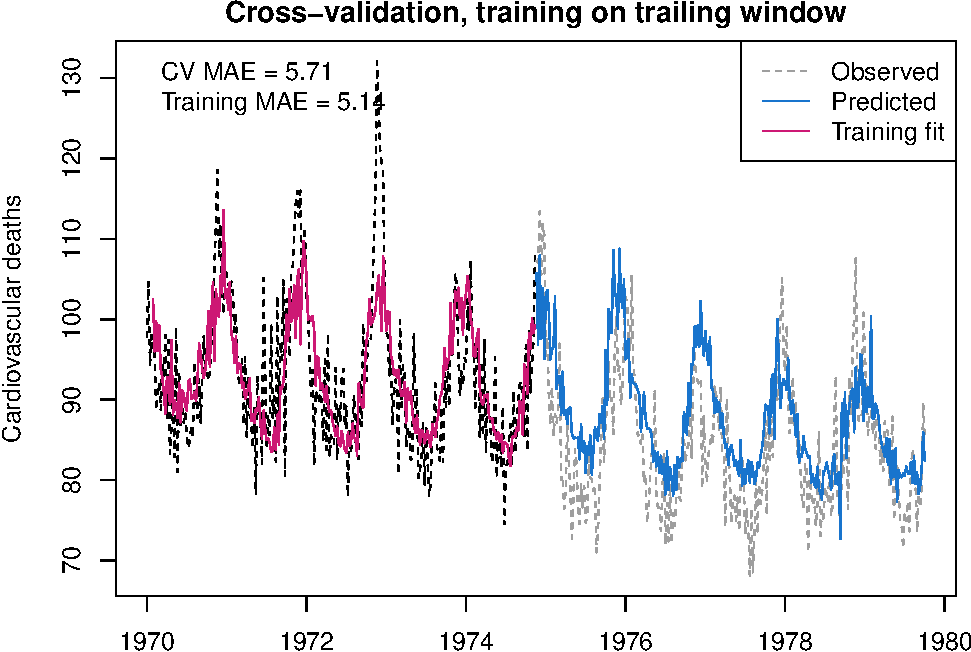
\includegraphics{homework2_files/figure-latex/unnamed-chunk-2-1.pdf}

\begin{enumerate}
\def\labelenumi{\arabic{enumi}.}
\setcounter{enumi}{12}
\tightlist
\item
  (2 pts) Repeat the same exercise as in Q12 but now with multiple lags
  per variable: use lags 4, 8, 12 for each of particulate level and
  temperature (thus 6 features in total). Did the training MAE go down?
  Did the cross-validated MAE go down? Discuss. Hint: you may find it
  useful to know that \texttt{lm()} can take a predictor matrix, as in
  \texttt{lm(y\ \textasciitilde{}\ x)} where \texttt{x} is a matrix; in
  this problem, you can form the predictor matrix by calling
  \texttt{cbind()} on the lagged feature vectors.
\end{enumerate}

\begin{Shaded}
\begin{Highlighting}[]
\CommentTok{\# CODE GOES HERE}

\CommentTok{\# Define lag sizes and initialize vectors}
\NormalTok{lags }\OtherTok{=} \FunctionTok{c}\NormalTok{(}\DecValTok{4}\NormalTok{, }\DecValTok{8}\NormalTok{, }\DecValTok{12}\NormalTok{)}
\NormalTok{n }\OtherTok{=} \FunctionTok{length}\NormalTok{(cmort)}
\NormalTok{n\_lags }\OtherTok{=} \FunctionTok{length}\NormalTok{(lags)}
\NormalTok{first\_half }\OtherTok{=} \DecValTok{1}\SpecialCharTok{:}\NormalTok{n }\SpecialCharTok{\textless{}=} \FunctionTok{floor}\NormalTok{(n}\SpecialCharTok{/}\DecValTok{2}\NormalTok{)}
\NormalTok{second\_half }\OtherTok{=} \DecValTok{1}\SpecialCharTok{:}\NormalTok{n }\SpecialCharTok{\textgreater{}} \FunctionTok{floor}\NormalTok{(n}\SpecialCharTok{/}\DecValTok{2}\NormalTok{)}

\NormalTok{cmort\_vec }\OtherTok{=} \FunctionTok{as.numeric}\NormalTok{(cmort)}
\NormalTok{tempr\_vec }\OtherTok{=} \FunctionTok{as.numeric}\NormalTok{(tempr)}
\NormalTok{part\_vec }\OtherTok{=} \FunctionTok{as.numeric}\NormalTok{(part)}

\CommentTok{\# Create matrix for all lags}
\NormalTok{mat }\OtherTok{=}\NormalTok{ dplyr}\SpecialCharTok{::}\FunctionTok{lag}\NormalTok{(part\_vec, lags[}\DecValTok{1}\NormalTok{])}
\NormalTok{mat }\OtherTok{=} \FunctionTok{cbind}\NormalTok{(mat, dplyr}\SpecialCharTok{::}\FunctionTok{lag}\NormalTok{(tempr\_vec, lags[}\DecValTok{1}\NormalTok{]))}

\ControlFlowTok{for}\NormalTok{ (i }\ControlFlowTok{in} \DecValTok{2}\SpecialCharTok{:}\NormalTok{n\_lags) \{}
\NormalTok{  mat }\OtherTok{=} \FunctionTok{cbind}\NormalTok{(mat, dplyr}\SpecialCharTok{::}\FunctionTok{lag}\NormalTok{(part\_vec, lags[i]))}
\NormalTok{  mat }\OtherTok{=} \FunctionTok{cbind}\NormalTok{(mat, dplyr}\SpecialCharTok{::}\FunctionTok{lag}\NormalTok{(tempr\_vec, lags[i]))}
\NormalTok{\}}

\CommentTok{\# Adjust the prediction part}
\NormalTok{t0 }\OtherTok{=} \FunctionTok{floor}\NormalTok{(n}\SpecialCharTok{/}\DecValTok{2}\NormalTok{)}
\NormalTok{yhat\_trailing }\OtherTok{=} \FunctionTok{rep}\NormalTok{(}\ConstantTok{NA}\NormalTok{, n }\SpecialCharTok{{-}}\NormalTok{ t0)}
\NormalTok{w }\OtherTok{=} \DecValTok{200} \CommentTok{\# Trailing window length}

\ControlFlowTok{for}\NormalTok{ (t }\ControlFlowTok{in}\NormalTok{ (t0}\SpecialCharTok{+}\DecValTok{1}\NormalTok{)}\SpecialCharTok{:}\NormalTok{n) \{}
\NormalTok{  reg\_trailing }\OtherTok{=} \FunctionTok{lm}\NormalTok{(cmort\_vec }\SpecialCharTok{\textasciitilde{}}\NormalTok{ .,}
                    \FunctionTok{data.frame}\NormalTok{(mat),}
                    \AttributeTok{subset =}\NormalTok{ (}\DecValTok{1}\SpecialCharTok{:}\NormalTok{n) }\SpecialCharTok{\textless{}=}\NormalTok{ t }\SpecialCharTok{{-}} \DecValTok{4} \SpecialCharTok{\&}\NormalTok{ (}\DecValTok{1}\SpecialCharTok{:}\NormalTok{n) }\SpecialCharTok{\textgreater{}}\NormalTok{ t }\SpecialCharTok{{-}}\NormalTok{ w }\SpecialCharTok{{-}} \DecValTok{4}\NormalTok{)}
  
\NormalTok{  yhat\_trailing[t }\SpecialCharTok{{-}}\NormalTok{ t0] }\OtherTok{=} \FunctionTok{predict}\NormalTok{(}
\NormalTok{    reg\_trailing,}
    \AttributeTok{newdata =} \FunctionTok{data.frame}\NormalTok{(}\FunctionTok{t}\NormalTok{(mat[t, ]))}
\NormalTok{  )}
\NormalTok{\}}

\NormalTok{mae\_trailing }\OtherTok{=} \FunctionTok{mean}\NormalTok{(}\FunctionTok{abs}\NormalTok{(cmort[second\_half] }\SpecialCharTok{{-}}\NormalTok{ yhat\_trailing), }\AttributeTok{na.rm =} \ConstantTok{TRUE}\NormalTok{)}

\CommentTok{\# Now, for the initial training set}
\NormalTok{reg\_first\_half }\OtherTok{=} \FunctionTok{lm}\NormalTok{(cmort\_vec }\SpecialCharTok{\textasciitilde{}}\NormalTok{ ., }\FunctionTok{data.frame}\NormalTok{(mat), }\AttributeTok{subset =}\NormalTok{ first\_half)}

\NormalTok{training\_fitted }\OtherTok{=} \FunctionTok{predict}\NormalTok{(reg\_first\_half, }\AttributeTok{newdata =} \FunctionTok{data.frame}\NormalTok{(mat[first\_half, ]))}

\NormalTok{mae\_training }\OtherTok{=} \FunctionTok{mean}\NormalTok{(}\FunctionTok{abs}\NormalTok{(cmort[first\_half] }\SpecialCharTok{{-}}\NormalTok{ training\_fitted), }\AttributeTok{na.rm =} \ConstantTok{TRUE}\NormalTok{)}

\CommentTok{\# Plot}
\FunctionTok{par}\NormalTok{(}\AttributeTok{mar =} \FunctionTok{c}\NormalTok{(}\DecValTok{2}\NormalTok{, }\DecValTok{4}\NormalTok{, }\DecValTok{2}\NormalTok{, }\FloatTok{0.5}\NormalTok{))}
\FunctionTok{plot}\NormalTok{(}\FunctionTok{time}\NormalTok{(cmort)[first\_half], cmort[first\_half], }\AttributeTok{type =} \StringTok{"l"}\NormalTok{, }
     \AttributeTok{xlim =} \FunctionTok{range}\NormalTok{(}\FunctionTok{time}\NormalTok{(cmort)), }\AttributeTok{ylim =} \FunctionTok{range}\NormalTok{(cmort),}
     \AttributeTok{xlab =} \StringTok{""}\NormalTok{, }\AttributeTok{ylab =} \StringTok{"Cardiovascular deaths"}\NormalTok{, }
     \AttributeTok{main =} \StringTok{"Cross{-}validation, training on trailing window"}\NormalTok{, }\AttributeTok{lty =} \DecValTok{2}\NormalTok{)}
\FunctionTok{lines}\NormalTok{(}\FunctionTok{time}\NormalTok{(cmort)[second\_half], cmort[second\_half], }\AttributeTok{col =} \DecValTok{8}\NormalTok{, }\AttributeTok{lty =} \DecValTok{2}\NormalTok{)}
\FunctionTok{lines}\NormalTok{(}\FunctionTok{time}\NormalTok{(cmort)[second\_half], yhat\_trailing, }\AttributeTok{col =} \DecValTok{4}\NormalTok{)}
\FunctionTok{lines}\NormalTok{(}\FunctionTok{time}\NormalTok{(cmort)[first\_half], training\_fitted, }\AttributeTok{col =} \DecValTok{6}\NormalTok{, }\AttributeTok{lty =} \DecValTok{1}\NormalTok{)}
\FunctionTok{legend}\NormalTok{(}\StringTok{"topright"}\NormalTok{, }\AttributeTok{legend =} \FunctionTok{c}\NormalTok{(}\StringTok{"Observed"}\NormalTok{, }\StringTok{"Predicted"}\NormalTok{, }\StringTok{"Training fit"}\NormalTok{), }
       \AttributeTok{lty =} \FunctionTok{c}\NormalTok{(}\DecValTok{2}\NormalTok{, }\DecValTok{1}\NormalTok{, }\DecValTok{1}\NormalTok{), }\AttributeTok{col =} \FunctionTok{c}\NormalTok{(}\DecValTok{8}\NormalTok{, }\DecValTok{4}\NormalTok{, }\DecValTok{6}\NormalTok{))}
\FunctionTok{legend}\NormalTok{(}\StringTok{"topleft"}\NormalTok{, }\AttributeTok{legend =} \FunctionTok{c}\NormalTok{(}\FunctionTok{paste}\NormalTok{(}\StringTok{"CV MAE ="}\NormalTok{, }\FunctionTok{round}\NormalTok{(mae\_trailing, }\DecValTok{2}\NormalTok{)), }
                             \FunctionTok{paste}\NormalTok{(}\StringTok{"Training MAE ="}\NormalTok{, }\FunctionTok{round}\NormalTok{(mae\_training, }\DecValTok{2}\NormalTok{))),}
       \AttributeTok{bty =} \StringTok{"n"}\NormalTok{)}
\end{Highlighting}
\end{Shaded}

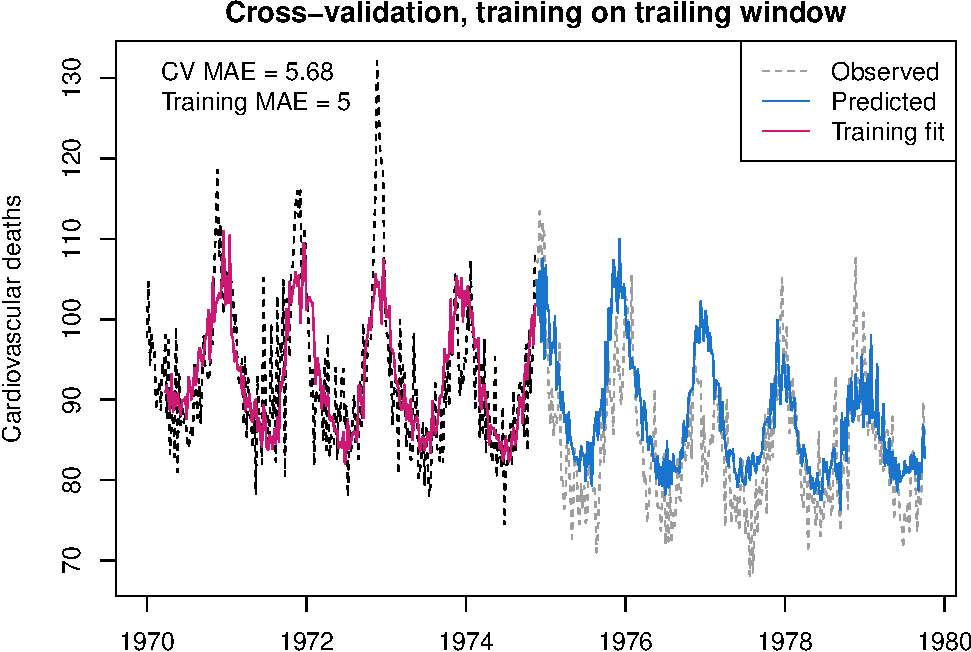
\includegraphics{homework2_files/figure-latex/unnamed-chunk-3-1.pdf}

\begin{enumerate}
\def\labelenumi{\arabic{enumi}.}
\setcounter{enumi}{13}
\tightlist
\item
  (2 pts) Repeat once more the same exercise as in the last question but
  but now with many lags per variable: use lags 4, 5, \ldots, through 50
  for each of particulate level and temperature (thus 47 x 2 = 94
  features in total). Did the training MAE go down? Did the
  cross-validated MAE go down? Are you surprised? Discuss.
\end{enumerate}

\begin{Shaded}
\begin{Highlighting}[]
\CommentTok{\# CODE GOES HERE}

\NormalTok{lags }\OtherTok{=} \FunctionTok{seq}\NormalTok{(}\DecValTok{4}\SpecialCharTok{:}\DecValTok{50}\NormalTok{)}
\NormalTok{n }\OtherTok{=} \FunctionTok{length}\NormalTok{(cmort)}
\NormalTok{n\_lags }\OtherTok{=} \FunctionTok{length}\NormalTok{(lags)}
\NormalTok{first\_half }\OtherTok{=} \DecValTok{1}\SpecialCharTok{:}\NormalTok{n }\SpecialCharTok{\textless{}=} \FunctionTok{floor}\NormalTok{(n}\SpecialCharTok{/}\DecValTok{2}\NormalTok{)}
\NormalTok{second\_half }\OtherTok{=} \DecValTok{1}\SpecialCharTok{:}\NormalTok{n }\SpecialCharTok{\textgreater{}} \FunctionTok{floor}\NormalTok{(n}\SpecialCharTok{/}\DecValTok{2}\NormalTok{)}

\NormalTok{cmort\_vec }\OtherTok{=} \FunctionTok{as.numeric}\NormalTok{(cmort)}
\NormalTok{tempr\_vec }\OtherTok{=} \FunctionTok{as.numeric}\NormalTok{(tempr)}
\NormalTok{part\_vec }\OtherTok{=} \FunctionTok{as.numeric}\NormalTok{(part)}

\CommentTok{\# Create matrix for all lags}
\NormalTok{mat }\OtherTok{=}\NormalTok{ dplyr}\SpecialCharTok{::}\FunctionTok{lag}\NormalTok{(part\_vec, lags[}\DecValTok{1}\NormalTok{])}
\NormalTok{mat }\OtherTok{=} \FunctionTok{cbind}\NormalTok{(mat, dplyr}\SpecialCharTok{::}\FunctionTok{lag}\NormalTok{(tempr\_vec, lags[}\DecValTok{1}\NormalTok{]))}

\ControlFlowTok{for}\NormalTok{ (i }\ControlFlowTok{in} \DecValTok{2}\SpecialCharTok{:}\NormalTok{n\_lags) \{}
\NormalTok{  mat }\OtherTok{=} \FunctionTok{cbind}\NormalTok{(mat, dplyr}\SpecialCharTok{::}\FunctionTok{lag}\NormalTok{(part\_vec, lags[i]))}
\NormalTok{  mat }\OtherTok{=} \FunctionTok{cbind}\NormalTok{(mat, dplyr}\SpecialCharTok{::}\FunctionTok{lag}\NormalTok{(tempr\_vec, lags[i]))}
\NormalTok{\}}

\CommentTok{\# Adjust the prediction part}
\NormalTok{t0 }\OtherTok{=} \FunctionTok{floor}\NormalTok{(n}\SpecialCharTok{/}\DecValTok{2}\NormalTok{)}
\NormalTok{yhat\_trailing }\OtherTok{=} \FunctionTok{rep}\NormalTok{(}\ConstantTok{NA}\NormalTok{, n }\SpecialCharTok{{-}}\NormalTok{ t0)}
\NormalTok{w }\OtherTok{=} \DecValTok{200} \CommentTok{\# Trailing window length}

\ControlFlowTok{for}\NormalTok{ (t }\ControlFlowTok{in}\NormalTok{ (t0}\SpecialCharTok{+}\DecValTok{1}\NormalTok{)}\SpecialCharTok{:}\NormalTok{n) \{}
\NormalTok{  reg\_trailing }\OtherTok{=} \FunctionTok{lm}\NormalTok{(cmort\_vec }\SpecialCharTok{\textasciitilde{}}\NormalTok{ .,}
                    \FunctionTok{data.frame}\NormalTok{(mat),}
                    \AttributeTok{subset =}\NormalTok{ (}\DecValTok{1}\SpecialCharTok{:}\NormalTok{n) }\SpecialCharTok{\textless{}=}\NormalTok{ t }\SpecialCharTok{{-}} \DecValTok{4} \SpecialCharTok{\&}\NormalTok{ (}\DecValTok{1}\SpecialCharTok{:}\NormalTok{n) }\SpecialCharTok{\textgreater{}}\NormalTok{ t }\SpecialCharTok{{-}}\NormalTok{ w }\SpecialCharTok{{-}} \DecValTok{4}\NormalTok{)}
  
\NormalTok{  yhat\_trailing[t }\SpecialCharTok{{-}}\NormalTok{ t0] }\OtherTok{=} \FunctionTok{predict}\NormalTok{(}
\NormalTok{    reg\_trailing,}
    \AttributeTok{newdata =} \FunctionTok{data.frame}\NormalTok{(}\FunctionTok{t}\NormalTok{(mat[t, ]))}
\NormalTok{  )}
\NormalTok{\}}

\NormalTok{mae\_trailing }\OtherTok{=} \FunctionTok{mean}\NormalTok{(}\FunctionTok{abs}\NormalTok{(cmort[second\_half] }\SpecialCharTok{{-}}\NormalTok{ yhat\_trailing), }\AttributeTok{na.rm =} \ConstantTok{TRUE}\NormalTok{)}

\CommentTok{\# Now, for the initial training set}
\NormalTok{reg\_first\_half }\OtherTok{=} \FunctionTok{lm}\NormalTok{(cmort\_vec }\SpecialCharTok{\textasciitilde{}}\NormalTok{ ., }\FunctionTok{data.frame}\NormalTok{(mat), }\AttributeTok{subset =}\NormalTok{ first\_half)}

\NormalTok{training\_fitted }\OtherTok{=} \FunctionTok{predict}\NormalTok{(reg\_first\_half, }\AttributeTok{newdata =} \FunctionTok{data.frame}\NormalTok{(mat[first\_half, ]))}

\NormalTok{mae\_training }\OtherTok{=} \FunctionTok{mean}\NormalTok{(}\FunctionTok{abs}\NormalTok{(cmort[first\_half] }\SpecialCharTok{{-}}\NormalTok{ training\_fitted), }\AttributeTok{na.rm =} \ConstantTok{TRUE}\NormalTok{)}

\CommentTok{\# Plot}
\FunctionTok{par}\NormalTok{(}\AttributeTok{mar =} \FunctionTok{c}\NormalTok{(}\DecValTok{2}\NormalTok{, }\DecValTok{4}\NormalTok{, }\DecValTok{2}\NormalTok{, }\FloatTok{0.5}\NormalTok{))}
\FunctionTok{plot}\NormalTok{(}\FunctionTok{time}\NormalTok{(cmort)[first\_half], cmort[first\_half], }\AttributeTok{type =} \StringTok{"l"}\NormalTok{, }
     \AttributeTok{xlim =} \FunctionTok{range}\NormalTok{(}\FunctionTok{time}\NormalTok{(cmort)), }\AttributeTok{ylim =} \FunctionTok{range}\NormalTok{(cmort),}
     \AttributeTok{xlab =} \StringTok{""}\NormalTok{, }\AttributeTok{ylab =} \StringTok{"Cardiovascular deaths"}\NormalTok{, }
     \AttributeTok{main =} \StringTok{"Cross{-}validation, training on trailing window"}\NormalTok{, }\AttributeTok{lty =} \DecValTok{2}\NormalTok{)}
\FunctionTok{lines}\NormalTok{(}\FunctionTok{time}\NormalTok{(cmort)[second\_half], cmort[second\_half], }\AttributeTok{col =} \DecValTok{8}\NormalTok{, }\AttributeTok{lty =} \DecValTok{2}\NormalTok{)}
\FunctionTok{lines}\NormalTok{(}\FunctionTok{time}\NormalTok{(cmort)[second\_half], yhat\_trailing, }\AttributeTok{col =} \DecValTok{4}\NormalTok{)}
\FunctionTok{lines}\NormalTok{(}\FunctionTok{time}\NormalTok{(cmort)[first\_half], training\_fitted, }\AttributeTok{col =} \DecValTok{6}\NormalTok{, }\AttributeTok{lty =} \DecValTok{1}\NormalTok{)}
\FunctionTok{legend}\NormalTok{(}\StringTok{"topright"}\NormalTok{, }\AttributeTok{legend =} \FunctionTok{c}\NormalTok{(}\StringTok{"Observed"}\NormalTok{, }\StringTok{"Predicted"}\NormalTok{, }\StringTok{"Training fit"}\NormalTok{), }
       \AttributeTok{lty =} \FunctionTok{c}\NormalTok{(}\DecValTok{2}\NormalTok{, }\DecValTok{1}\NormalTok{, }\DecValTok{1}\NormalTok{), }\AttributeTok{col =} \FunctionTok{c}\NormalTok{(}\DecValTok{8}\NormalTok{, }\DecValTok{4}\NormalTok{, }\DecValTok{6}\NormalTok{))}
\FunctionTok{legend}\NormalTok{(}\StringTok{"topleft"}\NormalTok{, }\AttributeTok{legend =} \FunctionTok{c}\NormalTok{(}\FunctionTok{paste}\NormalTok{(}\StringTok{"CV MAE ="}\NormalTok{, }\FunctionTok{round}\NormalTok{(mae\_trailing, }\DecValTok{2}\NormalTok{)), }
                             \FunctionTok{paste}\NormalTok{(}\StringTok{"Training MAE ="}\NormalTok{, }\FunctionTok{round}\NormalTok{(mae\_training, }\DecValTok{2}\NormalTok{))),}
       \AttributeTok{bty =} \StringTok{"n"}\NormalTok{)}
\end{Highlighting}
\end{Shaded}

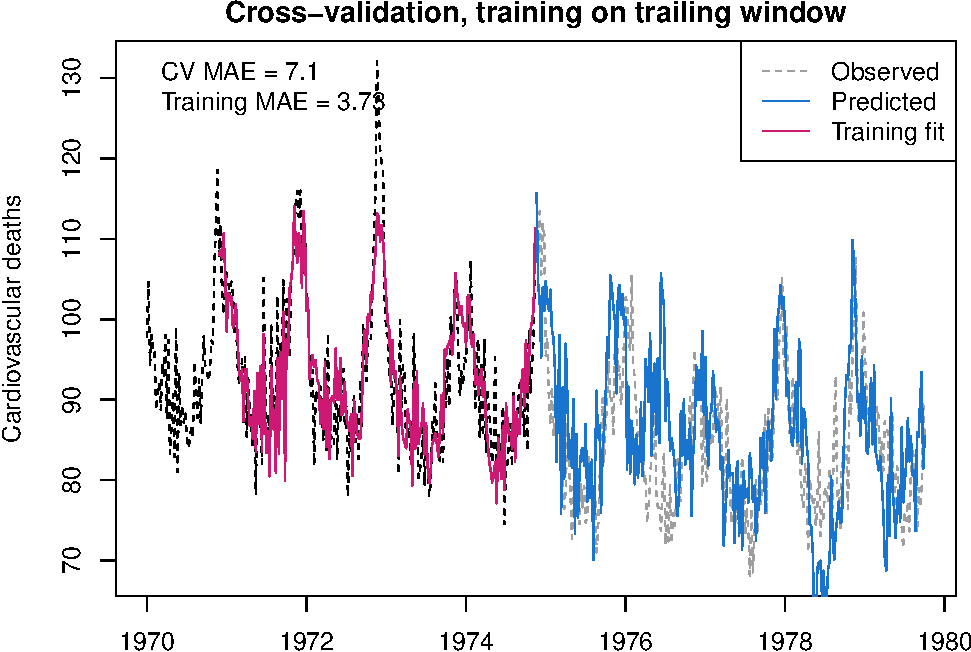
\includegraphics{homework2_files/figure-latex/unnamed-chunk-4-1.pdf}

\hypertarget{more-features-the-merrier}{%
\section{More features, the merrier?}\label{more-features-the-merrier}}

\begin{enumerate}
\def\labelenumi{\arabic{enumi}.}
\setcounter{enumi}{14}
\tightlist
\item
  (2 pts) Let \(y_i\) be an arbitrary response, and \(x_i \in \R^p\) be
  an arbitrary feature vector, for \(i = 1,\dots,n\). Let \[
  \tilde{x}_i = (x_{i1}, \dots, x_{ip}, \tilde{x}_{i,p+1}),\quad i = 1,\dots,n
  \] be the result of appending one more feature. Let \(\hat{y}_i\)
  denote the fitted values from the regression of \(y_i\) on \(x_i\),
  and let \(\tilde{y}_i\) denote the fitted values from the regression
  of \(y_i\) on \(\tilde{x}_i\). Prove that \[
  \sum_{i=1}^n (y_i - \tilde{y}_i)^2 \leq \sum_{i=1}^n (y_i - \hat{y}_i)^2.
  \] In other words, \emph{the training MSE will never get worse as we
  add features} to a given sample regression problem.
\end{enumerate}

SOLUTION GOES HERE

Assume for the sake of contradiction that the training MSE
\[\sum_{i=1}^n (y_i - \tilde{y}_i)^2 > \sum_{i=1}^n (y_i - \hat{y}_i)^2.\]
However, notice we can take \(\tilde{\beta}\) to be \(\hat{\beta}\) and
appending \(0\)'s to the end of \(\tilde{\beta}\) to make it a
\(p+1\)-dimensional vector. Then,
\(\tilde{y} = X\tilde{\beta} = X\hat{\beta} = \hat{y}\). Hence,
\[\sum_{i=1}^n (y_i - \tilde{y}_i)^2 = \sum_{i=1}^n (y_i - \hat{y}_i)^2,\]
which contradicts our assumption. Therefore, the training MSE is always
less than or equal to the test MSE.

\begin{enumerate}
\def\labelenumi{\arabic{enumi}.}
\setcounter{enumi}{15}
\tightlist
\item
  (2 pts) How many linearly independent features do we need (how large
  should \(p\) be) in order to achieve a perfect training accuracy,
  i.e., training MSE of zero? Why?
\end{enumerate}

SOLUTION GOES HERE

There need to be \(n\) linearly independent features, \(p=n\). For MSE
to be zero, the \(\ell_2\) norm \(||y - \hat{y}||_2 = 0\), which means
\(y = \hat{y}\). Note that \(\hat{y} = X \hat{\beta}\), a linear
combination of the column vectors of \(X\). In order to make sure there
exists \(\hat{y}\) such that \(y = \hat{y}\) for all
\(y\in \mathbb{R}^n\), the column space of \(X\) needs to span the
entire space of \(\mathbb{R}^n\), which means the column space of \(X\)
needs to have dimension at least \(n = \dim y\). Then, notice there can
never be more than \(n\) linearly independent features, because the
dimension of the column space of \(X\) is at most \(n\).

\begin{enumerate}
\def\labelenumi{\arabic{enumi}.}
\setcounter{enumi}{16}
\tightlist
\item
  (Bonus) Implement an example in R in order to verify your answer to
  Q16 empirically. Extra bonus points if you do it on the cardiovascular
  mortality data, using enough lagged features. You should be able to
  plot the fitted values from the training set and see that they match
  the observations perfectly (and the CV predictions should be super
  wild looking).
\end{enumerate}

\begin{Shaded}
\begin{Highlighting}[]
\CommentTok{\# CODE GOES HERE}
\end{Highlighting}
\end{Shaded}


\end{document}
